\item[8] Using only three (3) D flip-flops and any strictly combinational devices available in Logisim's Gates, Plexers, and Arithmetic component libraries, construct a synchronous device with no external control inputs that continually generates the sequence of unsigned values: 16, 13, 27, 17, 12, 26, (repeat from 16).

  Hint: Observe the least significant 3 bits of each unsigned value, and use patterns from those to construct the complete numbers.
\\{\color{NavyBlue}
\\Since we can use any plexers and 3 D-flip-lops to store at most 8 states, we can make a plexer into a look-up table and make the flip-flop values reset to 0 when it reaches 6 (so we have state 0,1,2,3,4,5, in total 6 states). In other words:
\\
\\MUX table:
\\
\\\begin{tabular}{c c c | c}
    $Q2$ & $Q1$ & $Q0$ & Output in hex \\
    \hline
    0 & 0 & 0 & 10 \\
    0 & 0 & 1 & 0D \\
    0 & 1 & 0 & 1B \\
    0 & 1 & 1 & 11 \\
    1 & 0 & 0 & 0C \\
    1 & 0 & 1 & 1A \\
    1 & 1 & 0 & X \\
    1 & 1 & 1 & X \\
    \end{tabular}
    \\
    \\ Flip flop reset condition = $Q2 \land Q1$
    \\
    \\Note that there is a way to do this without MUX, with flip flop outputs as inputs to digital circuits where output is each binary digits. That requires constructing 5 3-inputs k-maps. However, the output values from MUX are constants, so they wouldn't be counted as external control inputs, so doing it through a circuit adds unneccessary complications.
    }
    \\
    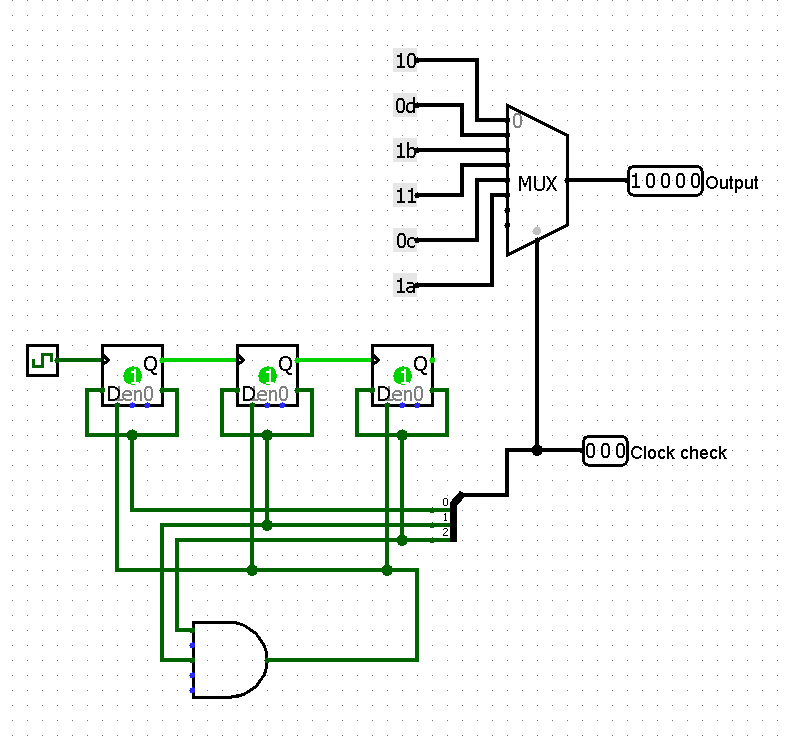
\includegraphics[width=5in]{q3.PNG}
    
\newpage